\chapter{Reciprocal Space}
\section{Definition and properties}
\dfn{Direction}{The direction in reciprocal space is defined by [$u, v, w$]}
\dfn{Planes}{The reciprocal planes are defined by ($h, k, l$)}
\clm{Properties of reciprocal space}{}{
\begin{enumerate}
    \setlength\itemsep{0pt}
    \item There are an infinite amount of lattice planes in a lattice.
    \item The set of all lattice planes contains only parallel lattice plains that contain all lattice points.
    \item The lattice plane closest to the origin cuts the coordinate axis in ($\frac{1}{h}, \frac{1}{k}, \frac{1}{l}$).
    \item There is always a lattice plane going through the origin.
\end{enumerate}
}

\section{Reciprocal space}
\subsection{Fourier transform of a periodic function}
As we know from section \ref{sec:trans_symm}, $V(\vec{r})$ is periodic. That's why we look at the FT of a periodic function.
\begin{align}
    f(x)    &= f(x + n\cdot a) \\
            &= \frac{a_0}{2} + \sum_{n=2}^{\infty}\left\{a_n\cos\frac{2\pi \cdot nx}{a} + b_n\sin\frac{2\pi \cdot nx}{a}\right\}\\
            &= \sum_{G}^{}{F(G)\cdot e^{iGx}}
\end{align}
Assuming for $n= -\infty \rightarrow \infty$
\begin{align}
    G &= \frac{2\pi}{a}n \\
    G\cdot a &= 2n\pi \\
    &\Rightarrow e^{iGa} = e^{2\pi n i} = 1
\end{align} \nt{For a reciporcal lattice number G: $[G] = \frac{1}{2}$}
Furthermore, the solutions for $a_n$ and $b_n$ are give by:
\begin{align}
    a_n &= \frac{2}{a_0} \int_{0}^{a} dx f(x)\cos\frac{2\pi \cdot nx}{a}\\
    b_n &= \frac{2}{a_0} \int_{0}^{a} dx f(x)\sin\frac{2\pi \cdot nx}{a}
\end{align}
\thm{Property of $F(G)$}{For a real sum: $F(-G) = F^*(G)$}
\qs{Using the FT for conversion of the lattice space to the recipocal space}{How does this translate to the lattice and potential?}
\ex{Using the FT for conversion of the lattice space to the recipocal space}{
	\tcbsidebyside[sidebyside adapt=center, blanker, sidebyside gap=-12cm,
               sidebyside align=middle]{\textit{1D:}}
	{
		\tcbsidebyside[sidebyside adapt=left, blanker, sidebyside gap=1cm,
				sidebyside align=top seam]{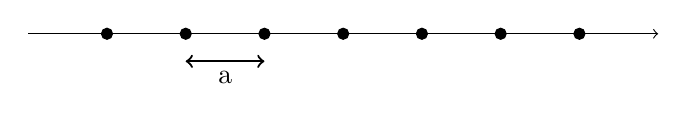
\begin{tikzpicture}
				\filldraw [black]	(0,0.35) circle (2pt)
									(1,0.35) circle (2pt)
									(2,0.35) circle (2pt)
									(3,0.35) circle (2pt)
									(4,0.35) circle (2pt)
									(5,0.35) circle (2pt)
									(6,0.35) circle (2pt);
				\draw [<->, black, thick]	(1, 0) to node [below]{a} (2, 0);
				\draw [->, black] (-1, 0.35) to (7, 0.35);
			\end{tikzpicture}}{\hspace{5pt}\textit{x}}

		\vspace{10pt}

		\tcbsidebyside[sidebyside adapt=left, blanker, sidebyside gap=1cm,
				sidebyside align=top seam]{\begin{tikzpicture}
				\filldraw [black]	(0,0.35) circle (2pt)
									(3.14,0.35) circle (2pt)
									(6.28,0.35) circle (2pt);
				\draw [<->, black, thick]	(0, 0) to node[below]{$\frac{2\pi}{a}$} (3.14, 0);
				\draw [->, black] (-1, 0.35) to (7, 0.35);
			\end{tikzpicture}}{\hspace{5pt}\textit{k}}
	}
	In lattice space we see that $V(x)$ is periode, $V(x) = V(x + na)$. $a$ is the lattice vector.
}
\subsection{Extension to 2D/3D}
Now, extending the above principle to 2D and 3D is straightforward but I'll still go over it.
\thm{}{
\begin{align}
	f(\vec{r}) &= f(x, y, z) = f(\vec{r} + \vec{T})\\
	&\Rightarrow e^{i\vec{G}\cdot\vec{T}} = 1 \qquad \forall \vec{T}
\end{align}

We define $\vec{r}$ as a vector in the lattice space and $\vec{T} = n_1\cdot\vec{a}_1 + n_2\cdot\vec{a}_2 + n_3\cdot\vec{a}_3$.
}
\begin{myproof}
\begin{align}
	f(\vec{r}) = \sum_{\vec{G}}^{}{&F(\vec{G})e^{i\vec{G}\cdot\vec{r}}} &\\
	\Rightarrow f(\vec{r} + \vec{T}) &= \sum_{\vec{G}}^{}{F{\vec{G}}e^i\vec{G}\cdot(\vec{r} + \vec{T})}\\
	&= \sum_{\vec{G}}^{}{F{\vec{G}}e^i\vec{G}\cdot(\vec{r})}\\
	e^{i\vec{G}\cdot\vec{T}} &= 1
\end{align}
\end{myproof}
By section \ref{sec:trans_symm} we can do step ($3.13$) because we know $f(\vec{r}) = f(\vec{r} + \vec{T})$ for a periodic lattice.
In general we can say: \begin{equation} F(\vec{G}) = \frac{1}{V}\int_{V}^{}f(\vec{r})e^{-i\vec{G}\cdot\vec{r}}d\vec{r} \end{equation}.

\section{Finding reciprocal lattice vectors}
As we know is $\vec{G}$ the reciprocal lattice vector, but how do we find this vector?\\
We know that: \begin{equation} e^{i\vec{G}\cdot\vec{T}} = 1 \Rightarrow \vec{G}\cdot\vec{T} = 2\pi n \label{eqn:def_of_G}\end{equation}
With
\begin{align}
	\vec{G} &= m_1\cdot\vec{b}_1 + m_2\cdot\vec{b}_2 + m_3\cdot\vec{b}_3 \\
	\vec{T} &= n_1\cdot\vec{a}_1 + n_2\cdot\vec{a}_2 + n_3\cdot\vec{a}_3 \\
	n &\rightarrow \delta_{ij} = \left\{
		\begin{array}{lr}
			1 & \text{if } i = j \\
			0 & \text{if } i \neq j
		\end{array}
	\right\label{eqn:deltarelation}
\end{align}
This results in the following definition: \begin{equation} \vec{a}_i \cdot \vec{b}_j = 2\pi\delta_{ij} \end{equation}
\nt{The reason for defining $\delta_{ij}$ as either $0$ or $1$ is to have orthogonal $\vec{a}_i$ and $\vec{b}_j$.}
Then the following vectors $\vec{b}_j$ span the reciprocal space $\vec{G}$. When satisfying relation ($3.20$), $\vec{b}_j$ can be described in function of $\vec{a}_i$:
\begin{align}
	\vec{b}_1 &= 2\pi\frac{\vec{a}_2\times\vec{a}_3}{\vec{a}_1\cdot(\vec{a}_2\times\vec{a}_3)} = \frac{2\pi}{V}(\vec{a}_2\times\vec{a}_3) \label{eqn:b1}\\
	\vec{b}_2 &= 2\pi\frac{\vec{a}_3\times\vec{a}_1}{\vec{a}_2\cdot(\vec{a}_3\times\vec{a}_1)} = \frac{2\pi}{V}(\vec{a}_3\times\vec{a}_1)\\
	\vec{b}_3 &= 2\pi\frac{\vec{a}_1\times\vec{a}_2}{\vec{a}_3\cdot(\vec{a}_1\times\vec{a}_2)} = \frac{2\pi}{V}(\vec{a}_1\times\vec{a}_2) \label{eqn:b3}\\
	&\Rightarrow \vec{G} = m_1\cdot\vec{b}_1 + m_2\cdot\vec{b}_2 + m_3\cdot\vec{b}_3
\end{align}
As we see describing $\vec{b}_j$ is a cyclic procedure.

\section{Properties of reciporcal spaces}
\clm{Property 1}{}{To every lattice plane ($h, k, l$) there is a reciprocal lattice vector perpendicular to htat plan and is give by $\vec{G} = h\cdot\vec{b}_1 + k\cdot\vec{b}_2 + l\cdot\vec{b}_3$.}
\begin{myproof}
	It is sufficient to show that the vector $\vec{R}$, perpendicular to the lattice plan ($h, k, l$), is parallel to $\vec{G}$. In order that: \begin{equation} \frac{\vec{R}}{\norm{\vec{R}}} = \frac{\vec{G}}{\norm{\vec{G}}} \end{equation}
	Then take a lattice plane ($h, k, l$):
	\begin{center}
	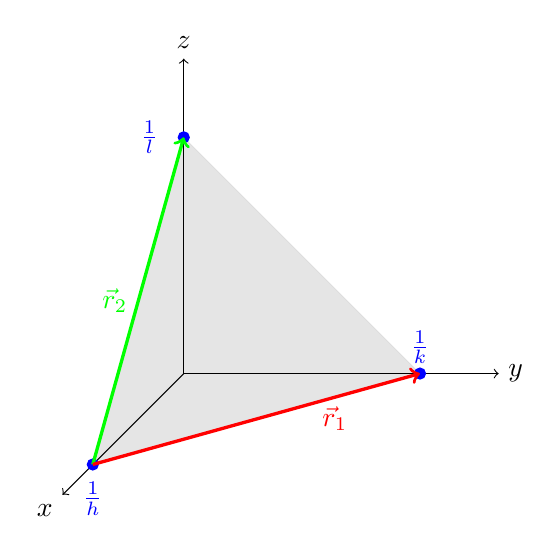
\begin{tikzpicture}
		\draw [->, black]	(0, 0, 0) to (0, 0, 4) node[anchor=north east]{$x$};
		\draw [->, black]	(0, 0, 0) to (0, 4, 0) node[above]{$z$};
		\draw [->, black]	(0, 0, 0) to (4, 0, 0) node[right]{$y$};

		\filldraw[draw=gray, opacity=0.1] (0, 0, 3) to (0, 3, 0) to (3, 0, 0);

		\filldraw[blue]	(0, 0, 3) circle (2pt);
		\filldraw[blue]	(0, 3, 0) circle (2pt);
		\filldraw[blue]	(3, 0, 0) circle (2pt);

		\draw [->, green, very thick]	(0, 0, 3) to node[left]{$\vec{r}_2$} (0, 3, 0);
		\draw [->, red, very thick]	(0, 0, 3) to node[right=7mm]{$\vec{r}_1$} (3, 0, 0);

		\draw [blue] (0, 3, 0) node[left=2mm] {$\frac{1}{l}$};
		\draw [blue] (3, 0, 0) node[above] {$\frac{1}{k}$};
		\draw [blue] (0, 0, 3) node[below=1mm] {$\frac{1}{h}$};
	\end{tikzpicture}
	\end{center}
	We define $\vec{r}_1 = \frac{\vec{a}_2}{k} - \frac{\vec{a}_1}{h}$ and $\vec{r}_2 = \frac{\vec{a}_3}{l} - \frac{\vec{a}_1}{h}$.
	The vector perpendiculas to the area spanned (gray) by $\vec{r}_1$ and $\vec{r}_2$ is given by $\vec{R} = \vec{r}_1 \times \vec{r}_2$. If we fill in the vectors according to the definitons, we get:
	\begin{align}
		\vec{R} &= \left\{\frac{\vec{a}_2}{k} - \frac{\vec{a}_1}{h}\right\} \times \left\{\frac{\vec{a}_3}{l} - \frac{\vec{a}_1}{h}\right\} \\
		&= \frac{\vec{a}_2}{k} \times \left\{\frac{\vec{a}_3}{l} - \frac{\vec{a}_1}{h} \right\} - \frac{\vec{a}_1}{h} \times \left\{\frac{\vec{a}_3}{l} - \frac{\vec{a}_1}{h} \right\} \label{eqn:determinant_R}\\
		&= C\cdot\vec{G} \\
		&\sim \vec{G}
	\end{align}

	And thus from
		\begin{align}
		\frac{\vec{G}}{\norm{\vec{G}}} &= \frac{\vec{R}}{\norm{\vec{R}}} \\
		&= \frac{C\cdot\vec{G}}{\norm{C\cdot\vec{G}}} \\
		&= \frac{C\cdot\vec{G}}{C\cdot\norm{\vec{G}}} = \frac{\vec{G}}{\norm{\vec{G}}}\\
		&\Rightarrow \vec{R} // \vec{G}\nonumber
		\end{align}
\end{myproof}
\nt{If you work out equation \ref{eqn:determinant_R} you get the formulas for $\vec{b}_j$, see equations \ref{eqn:b1} - \ref{eqn:b3}. Keep in mind that $\vec{a} \times -\vec{b} = \vec{b} \times \vec{a}$ and that distributivity is defined for cross products.}

\clm{Property 2}{}{The spacing d between the lattice plane closest to the origin and the origin itself is given by:
\begin{align}
	&\frac{2\pi}{\norm{\vec{G}}} \\
	\Rightarrow \norm{\vec{G}} &= \frac{2\pi}{d}
\end{align}}
\begin{myproof}
\begin{align}
	d &= \text{the distance betwee the ($h, k, l$) planes} \nonumber \\
	&= \frac{\vec{a}_1}{h}\cdot\frac{\vec{G}}{\norm{\vec{G}}} \\
	&= \frac{1}{h\norm{\vec{G}}}h\vec{a}_1\cdot\vec{b}_1 = \frac{2\pi}{\norm{\vec{G}}} \label{eqn:prop2simplification}
\end{align}
Step \ref{eqn:prop2simplification} uses the fact that $\vec{a}_i$ and $\vec{b}_j$ are perpendicular as per \ref{eqn:deltarelation}.
\end{myproof}

\clm{Property 3}{}{The direct lattice is the reciprocal of its own reciprocal lattice. Because switching the vectors in expression \ref{eqn:def_of_G} results in the same expression.}

\clm{Property 4}{}{The volume of a primitive unit cell of the reciprocal lattice is given by:
\begin{align}
	V_R &= \vec{b}_1\cdot(\vec{b}_2\times\vec{b}_3) \\
	&= \frac{8\pi^3}{V}
\end{align}
With $V = \vec{a}_1\cdot(\vec{a}_2\times\vec{a}_3)$, the volume of the direct lattice \textit{PUC}.}
\pagebreak
